\section{Many manoeuvres: sharp asymptotics}\label{sec:asym}

\subsection{Statements}
For $g>0$ let $N(g)$ be the least number of manoeuvres of a parking motion for the slot length $L=\ell+g$, with $N(g)=\infty$ if there is none.
By \cref{lem:monoL}, $N$ is non-increasing.
Under the hypotheses of \cref{thm:asym} no parked configuration exists when $L<\ell$: the argument of \cref{lem:confine}(ii) below gives $f(|\psi|)\le L-\ell$ for a function $f\ge0$.
Hence $\Lmin(n)\ge\ell$, and $\Lmin(n)=\ell+\inf\{g>0:\ N(g)\le n\}$.

\begin{theorem}\label{thm:mono}
$\Lmin(n)$ is non-increasing in $n$.
Under the hypotheses of \cref{thm:asym}, moreover $\ell<\Lmin(n)\le\Lmin(1)$ for every $n$, and $\Lmin(n)\to\ell$ as $n\to\infty$.
\end{theorem}

Some hypothesis such as $H<\ell$ is needed for $\Lmin(n)>\ell$.
If $\ell\le H$, a car can turn in the lane and drive nose-first straight down into the slot; it is then parked with heading $-\pi/2$ in a slot of length about $w<\ell$.

\begin{theorem}\label{thm:asym}
Assume the standing assumption $R>w/2$, $0<m<w$, $H<\ell$, $d_b\le b$, and
\begin{equation}\label{eq:mcond}
  m<\frac{2w\cos^2\psi_{\rm fit}}{1+2\cos\psi_{\rm fit}}
\end{equation}
(which holds, for instance, whenever $m\le w/2$ and $\ell\ge2w$). Put
\[
  r_*(u)=\begin{cases}\dfrac1{4R}, & 0\le u\le \tfrac w2,\\[8pt] \dfrac{R}{4\big(R^2-(u-\frac w2)^2\big)}, & \tfrac w2\le u\le w,\end{cases}
  \qquad K^2=\int_0^w\frac{\dd u}{r_*(u)}=4Rw-\frac{w^3}{6R}.
\]
Then $\lim_{g\downarrow0}g^2N(g)=K^2$; consequently $\sqrt n\,(\Lmin(n)-\ell)\to K$ as $n\to\infty$.
\end{theorem}

Here $u$ measures how far the car has been lifted out of the slot, and $g^2r_*(u)$ is the largest lift per manoeuvre achievable at height $u$, to leading order.
The two theorems are proved in \cref{sec:asym-proofs}.
The main steps:
\begin{enumerate}[nosep]
\item a \emph{confinement lemma}: until the car is almost out, the heading stays $O(g)$ along every exit;
\item an exact description of the free configurations in rescaled variables: a parallelogram (\emph{window});
\item a \emph{calibration}: a function $G$ on the window such that the lift in one manoeuvre is at most $g^2(r_*+\Delta G)$ up to $O(g^3)$;
\item a matching construction by tilted S-curves.
\end{enumerate}

\subsection{Rescaled variables}
Fix the slack $g\in(0,1]$ and write $L=\ell+g$.
For a configuration $q=(P,\psi)$ set
\[
  u=P_y-\tfrac w2-m,\qquad \xi=\frac{P_x-d_b}{g},\qquad \phi=\frac{\psi}{g}.
\]
For a level car, $u$ is the height of its curb-side edge above the curb-side edges of the parked cars.
A parked level car has $u\le0$, and a level car in the lane has $u\ge w$.
Along a manoeuvre of direction $d$,
\begin{equation}\label{eq:lift}
  \frac{\dd u}{\dd s}=d\sin\psi,\qquad \frac{\dd P_x}{\dd s}=d\cos\psi,\qquad\text{hence}\qquad \dd u=\tan\psi\,\dd P_x=g^2\,\frac{\tan\psi}{\psi}\,\phi\,\dd\xi .
\end{equation}
Moreover $\dd\phi/\dd\xi=\psi'/(d\cos\psi)\in[-1/(R\cos\psi),\,1/(R\cos\psi)]$.
So, to leading order, the rescaled state $(\xi,\phi)$ moves along curves of slope at most $1/(R\cos\psi)$ in absolute value; $\xi$ increases in forward manoeuvres and decreases in reverse ones.
The lift is the area-like integral $g^2\int\phi\,\dd\xi$.

\subsection{Confinement}

\begin{lemma}[confinement]\label{lem:confine}
Let $0<\delta\le w/4$.
Put $c=\max(4/\delta,\,4/(w-m))$, and choose $\psi_1\in(0,\delta/(2b)]$ so small that
\[
  (w-m\sec\psi_1)\Big(1-\frac{\psi_1^2}6\Big)-\frac{\ell\psi_1}2\ \ge\ \frac{w-m}2,\qquad \cos\psi_1>\frac mw,\qquad \frac{w\psi_1^2}{4}<\frac\delta4 .
\]
There is $g_0>0$ (depending on $\delta$ and the parameters) such that for $0<g\le g_0$:
\begin{enumerate}[label=(\roman*)]
\item no free configuration has $u\le w-\delta$ and $cg\le|\psi|\le\psi_1$;
\item every parked configuration has $|\psi|<cg$ (heading taken modulo $\pi$ as in \cref{lem:fit});
\item along every exit motion, $|\psi|<cg$ holds up to the first time $T_\delta$ at which $u\ge w-\delta$, and $T_\delta$ exists.
\end{enumerate}
\end{lemma}

\begin{proof}
(i) Let $q$ be free with $u\le w-\delta$ and $\psi\in[cg,\psi_1]$ (nose-up); the nose-down case is symmetric and treated at the end.
The corner heights are
\[
\begin{aligned}
  \cRC_y&=m+u+\tfrac w2(1-\cos\psi)-d_b\sin\psi, & \cFC_y&=m+u+\tfrac w2(1-\cos\psi)+b\sin\psi,\\
  \cRL_y&=m+u+w-\tfrac w2(1-\cos\psi)-d_b\sin\psi, & \cFL_y&=\cRL_y+\ell\sin\psi .
\end{aligned}
\]
The leftmost point is $\cRL$ and the rightmost is $\cFC$.
Since $\cRC_y\ge0$, we have $\cRL_y\ge w\cos\psi>m$, so $\cRL$ is never in the gap.

\emph{Case a: $\cFC_y\ge H$.}
Then $u\ge w-b\sin\psi-\tfrac w2(1-\cos\psi)>w-b\psi_1-\tfrac w4\psi_1^2>w-\delta$, which is excluded.

\emph{Case b: $\cFC_y\in(m,H)$ and $\cRL_y<H$.}
Both extreme corners lie in the band, so $\cFC_x\le L$ and $\cRL_x\ge0$.
This gives $\ell\cos\psi+w\sin\psi\le\ell+g$.
Using $\sin\psi\ge\psi(1-\psi^2/6)$ and $1-\cos\psi\le\psi^2/2$, we get $\psi\,\big(w(1-\psi_1^2/6)-\ell\psi_1/2\big)\le g$.
The bracket is at least $(w-m)/2$, so $\psi\le 2g/(w-m)<cg$, a contradiction.

\emph{Case c: $\cFC_y\in(m,H)$ and $\cRL_y\ge H$.}
The band part of the rear edge ends at height $H$, at the point with abscissa $P_x-d_b\sec\psi-(H-P_y)\tan\psi$, which must be $\ge0$.
Together with $\cFC_x\le L$ and $H-P_y=\tfrac w2-u$, this yields after multiplication by $\cos\psi$
\[
  \sin\psi\Big[\tfrac w2(1+\cos\psi)-u\Big]\ \le\ g\cos\psi+(1-\cos\psi)(b\cos\psi-d_b).
\]
Divide by $\sin\psi$ and use $u\le w-\delta$, $g\cot\psi\le g/\psi\le1/c\le\delta/4$ and $\tan(\psi/2)\le\psi\le\psi_1$.
This gives $\delta-\tfrac w4\psi_1^2\le\delta/4+b\psi_1\le\delta/4+\delta/2$, contradicting $w\psi_1^2/4<\delta/4$.

\emph{Case d: $\cFC_y\le m$.}
Then $u<0$, so $\cRL_y<H$ and $\cRL_x\ge0$.
The front edge rises from $\cFC$ to $\cFL$ with $\cFL_y=\cFC_y+w\cos\psi\in(m,H]$, so its point at height $m$ has abscissa $\cFC_x-(m-\cFC_y)\tan\psi\le L$.
Hence $\ell\cos\psi+w\sin\psi-m\tan\psi\le\ell+g$, and therefore $\psi\big[(w-m\sec\psi_1)(1-\psi_1^2/6)-\ell\psi_1/2\big]\le g$.
This again gives $\psi\le2g/(w-m)<cg$.

\emph{Nose-down, $\psi\in[-\psi_1,-cg]$, $a=|\psi|$.}
Now the leftmost point is $\cRC$ (height $m+u+\tfrac w2(1-\cos a)+d_b\sin a$), the rightmost is $\cFL$ (height $m+u+w-\tfrac w2(1-\cos a)-b\sin a$), and $\cFL_y\ge w\cos a>m$.
\begin{itemize}[nosep]
\item If $\cRC_y\ge H$, then $u>w-\delta$.
\item If both $\cRC$ and $\cFL$ lie in the band, we argue as in case b.
\item If $\cRC$ lies in the band and $\cFL_y\ge H$, the band part of the front edge ends at height $H$, at abscissa $P_x+b\sec a+(H-P_y)\tan a\le L$.
With $P_x\ge d_b\cos a+\tfrac w2\sin a$ this gives $\sin a\big[\tfrac w2(1+\cos a)-u\big]\le g\cos a-(1-\cos a)(b-d_b\cos a)\le g\cos a$.
This is excluded as in case c, here without the $b\psi_1$ term.
\item If $\cRC_y\le m$, then $u<0$ and the rear edge's point at height $m$ has abscissa $\cRC_x+(m-\cRC_y)\tan a\ge0$.
With $\cFL_x\le L$ this is case d.
\end{itemize}

(ii) A parked configuration has $|\psi|\le\psi_{\rm fit}$ by \cref{lem:fit}, and since its highest point is at most $H$, it has $u\le\frac w2(1-\cos\psi_{\rm fit})<w-\delta$.
Cases b and d, applied to $\psi\in(0,\psi_{\rm fit}]$, and their nose-down analogues for $\psi\in[-\psi_{\rm fit},0)$ give $f(|\psi|)\le g$, where $f(\psi):=(w-m\sec\psi)\sin\psi-\ell(1-\cos\psi)$.
Now $f$ is positive on $(0,\psi_{\rm fit}]$.
Indeed, $f(\psi)>0$ is equivalent to $w-m\sec\psi>\ell\tan(\psi/2)$; the left side decreases and the right side increases in $\psi$.
At $\psi_{\rm fit}$, using $\ell\tan(\psi_{\rm fit}/2)=\ell\sin\psi_{\rm fit}/(1+\cos\psi_{\rm fit})=(m+w(1-\cos\psi_{\rm fit}))/(1+\cos\psi_{\rm fit})$, the inequality reduces to \eqref{eq:mcond}.
Moreover $f(\psi)\ge\frac{w-m}2\psi$ on $(0,\psi_1]$.
(Cases b and d use $\cos\psi>m/w$ for $\psi\le\psi_{\rm fit}$; this follows from \eqref{eq:mcond}, since $2c_f^2/(1+2c_f)<c_f$ for $c_f=\cos\psi_{\rm fit}\in(0,1]$.)
Hence for $g<\min_{[\psi_1,\psi_{\rm fit}]}f$ every parked configuration has $|\psi|\le 2g/(w-m)<cg$.

(iii) Choose $g_0$ such that (ii) holds and $cg_0<\psi_1$.
Along an exit motion $\psi$ is continuous and starts in $(-cg,cg)$.
If $|\psi|$ reached $cg$ at a first time $t_1<T_\delta$, then $q(t_1)$ would violate (i).
At the end the car is in the lane, so its lowest point is at height $\ge H$.
If $|\psi|<cg$ there, then $u\ge w-\max(b,d_b)\,cg-\tfrac w2c^2g^2>w-\delta$ (decreasing $g_0$ if necessary); otherwise $T_\delta$ has already occurred.
Hence $T_\delta$ exists.
\end{proof}

\subsection{Windows}
From now on $0<g\le g_0$ and $|\psi|<cg$, so $|\phi|<c$.
For $k\in[0,w/2]$ introduce the sheared coordinate
\[
  \zeta_k=\xi+k\phi .
\]
\begin{lemma}[windows]\label{lem:windows}
There is a constant $A$ (depending on $\delta$ and the parameters) with the following property, after decreasing $g_0$ if necessary.
Let $q$ be free with $|\psi|<cg$ and $0\le u\le w-\delta$, and let $k\in[0,w/2]$ satisfy $k\ge u-\tfrac w2$.
Then $-Ag\le\zeta_k\le1+Ag$.
\end{lemma}

\begin{proof}
Since $|\psi|<cg$ and $0\le u\le w-\delta$, for $g$ small:
\begin{itemize}[nosep]
\item nose-up, the leftmost corner $\cRL$ is in the band or above $H$, and the rightmost corner $\cFC$ is in the band;
\item nose-down, the leftmost corner $\cRC$ is in the band, and the rightmost corner $\cFL$ is in the band or above $H$.
\end{itemize}
(A corner in the gap is never extreme in these cases.)
The exact constraints are therefore, for $\psi\ge0$,
\[
  P_x\ \ge\ \min\big(d_b\cos\psi+\tfrac w2\sin\psi,\ d_b\sec\psi+(\tfrac w2-u)\tan\psi\big),\qquad P_x\le L-b\cos\psi-\tfrac w2\sin\psi,
\]
and for $\psi<0$, with $a=|\psi|$,
\[
  P_x\ \ge\ d_b\cos a+\tfrac w2\sin a,\qquad P_x\ \le\ L-\min\big(b\cos a+\tfrac w2\sin a,\ b\sec a+(\tfrac w2-u)\tan a\big).
\]
In each case the first expression applies when the lane-side corner is in the band, the second when it is above $H$; in both cases we use the weaker of the two bounds.
Expanding to first order in $\psi$, with $O(g^2)$ remainders uniform in the stated ranges, these give
\[
  \xi\ \ge\ \min\big(\tfrac w2,\tfrac w2-u\big)\phi-Ag,\quad \xi\le1-\tfrac w2\phi+Ag\qquad(\phi\ge0),
\]
\[
  \xi\ \ge\ \tfrac w2|\phi|-Ag,\quad \xi\le1-\min\big(\tfrac w2,\tfrac w2-u\big)|\phi|+Ag\qquad(\phi<0).
\]
Adding $k\phi$ and using $\tfrac w2-u+k\ge0$ and $k\le\tfrac w2$ gives the claim.
\end{proof}

\begin{remark}\label{rem:parallelogram}
For $u\ge w/2$ and $k=u-w/2$, the leading-order window is exactly the parallelogram
\[
  \Pi_u=\{(\zeta,\phi):\ 0\le\zeta\le1,\ 0\le\zeta+(w-u)\phi\le1\}.
\]
Its vertices are $(0,0)$, $(1,0)$, $(0,1/(w-u))$ and $(1,-1/(w-u))$.
For $u\le w/2$ and $k=0$ it is the parallelogram with vertices $(0,0)$, $(1,0)$, $(\frac{w/2-u}{w-u},\frac1{w-u})$, $(\frac{w/2}{w-u},-\frac1{w-u})$, contained in the strip $0\le\xi\le1$.
In both cases the leading-order window is
\[
  \Pi_u=\big\{0\le\xi+(u-\tfrac w2)\phi\le1\big\}\cap\big\{0\le\xi+\tfrac w2\phi\le1\big\}\qquad(0\le u\le w).
\]
It lies in the strip $\{0\le\zeta_k\le1\}$ exactly when $k\in[u-\frac w2,\frac w2]$.
Since $r_k$ increases with $|k|$, the choice $k(u)=\max(0,u-\frac w2)$ in \cref{lem:calib} below is the best admissible one, which is why the lower and upper bounds match.
\end{remark}

\begin{figure}[ht]
\centering
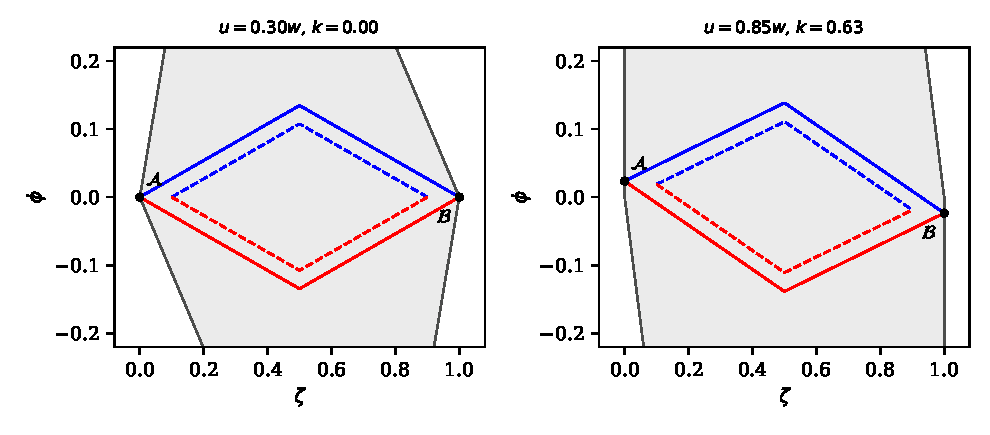
\includegraphics[width=\textwidth]{figures/fig_window.pdf}
\caption{Rescaled windows (grey, partly shown) and ideal loops for the typical car: upper branch (forward S-curve) in blue, lower branch (reverse S-curve) in red.
Solid: $\lambda=1$; dashed: $\lambda=0.8$.
Left: $u=0.3w$, untilted loop.
Right: $u=0.85w$; the window is slanted and the optimal loop is tilted by $\varpi(u)$.}
\label{fig:window}
\end{figure}

\subsection{Calibration}
Write $s_\pm(k)=1/(R\pm k)$ and
\[
  r_k=\frac{s_+(k)+s_-(k)}8=\frac{R}{4(R^2-k^2)},\qquad G_k(q)=(\xi-\tfrac12)\phi+\tfrac k2\phi^2 .
\]
Note that $r_*(u)=r_{k(u)}$ with $k(u)=\max(0,u-\tfrac w2)$.

\begin{lemma}[calibration]\label{lem:calib}
There is a constant $B$ (depending on $\delta$ and the parameters) such that, after decreasing $g_0$ if necessary, the following holds for $0<g\le g_0$ and $k\in[0,w/2]$.
Let $q$ be a manoeuvre, or a sub-interval of one, along which $|\psi|<cg$ and $\zeta_k\in[-Ag,1+Ag]$.
Then
\[
  \Delta u\ \le\ g^2\big(r_k+\Delta G_k\big)+Bg^3 ,
\]
where $\Delta$ denotes the increment from start to end.
\end{lemma}

\begin{proof}
By \eqref{eq:lift}, $\Delta u=g^2\int\phi\,\dd\xi+g^2\int(\tfrac{\tan\psi}{\psi}-1)\phi\,\dd\xi$.
Here $\xi=\zeta_k-k\phi$ is monotone along a manoeuvre with total variation at most $1+2Ag+wc$, and the second integrand is $O(g^2)$; so the second term is $O(g^4)$.
For the main term, $\dd\xi=\dd\zeta_k-k\,\dd\phi$, so
\[
  \int\phi\,\dd\xi=\Delta\Big[(\zeta_k-\tfrac12)\phi-\tfrac k2\phi^2\Big]-\int(\zeta_k-\tfrac12)\,\dd\phi=\Delta G_k-\int(\zeta_k-\tfrac12)\,\dd\phi .
\]
Along the manoeuvre, $\frac{\dd\zeta_k}{\dd s}=(d\cos\psi+k\psi')/g$, which has the sign of $d$ because $k|\psi'|\le w/(2R)<\cos\psi$ for small $g$.
So $\zeta_k$ is monotone, and $\dd\phi=\sigma\,\dd\zeta_k$ with
\[
  \sigma=\frac{\psi'}{d\cos\psi+k\psi'}\in\Big[-\frac1{R\cos\psi-k},\ \frac1{R\cos\psi+k}\Big].
\]
For reverse manoeuvres put $t=-\psi'$; the map $t\mapsto t/(\cos\psi+kt)$ is increasing.
Write $s'_\pm$ for the supremum of $1/(R\cos\psi\pm k)$ over the manoeuvre; then $s'_\pm=s_\pm(1+O(g^2))$.

For a forward manoeuvre ($\dd\zeta_k>0$) the integrand $-(\zeta_k-\frac12)\sigma$ is at most $s'_+(\frac12-\zeta_k)^+ + s'_-(\zeta_k-\frac12)^+$.
For a reverse manoeuvre we write $-\int(\zeta_k-\frac12)\sigma\,\dd\zeta_k=\int(\zeta_k-\frac12)\sigma\,|\dd\zeta_k|$.
Its integrand is at most $s'_+(\zeta_k-\frac12)^+ + s'_-(\frac12-\zeta_k)^+$.
In both cases $\zeta_k$ sweeps a sub-interval of $[-Ag,1+Ag]$ once.
Hence
\[
  -\int(\zeta_k-\tfrac12)\,\dd\phi\ \le\ (s'_++s'_-)\int_{-Ag}^{1/2}(\tfrac12-z)\,\dd z\ =\ \frac{(1+2Ag)^2}8\,(s'_++s'_-)=r_k+O(g).\qedhere
\]
\end{proof}

The bound is sharp, and $\sigma=\kappa/(\cos\psi+k\kappa)$ depends only on the steering.
In a forward manoeuvre equality requires $\sigma=s_+$ (full left lock) while $\zeta_k<\frac12$ and $\sigma=-s_-$ (full right lock) afterwards.
In a reverse manoeuvre, where $\zeta_k$ decreases, it requires $\sigma=s_+$ (full left lock) while $\zeta_k>\frac12$ and $\sigma=-s_-$ (full right lock) afterwards.
Each manoeuvre must also sweep the whole window.
This is exactly the S-curve of the construction in \cref{sec:construction}.
